\section{Architecture} \label{sec:architecture}
\subsection{Overview} \label{sec:architecture:overview}
In simple terms, a BF machine consists of an array of memory-cells, together with a pointer pointing to one of these cells. The pointer can move along the array while modifying its contents one step at a time. An example of this representation in some intermediate state is shown in Figure \ref{fig:simplerepresentation}. Consider the BF program ``\texttt{>>>>>+.}'', applied to the initial conditions shown in the example. The pointer would take 5 steps to the right, landing on cell 9 which contains the number 41. It will then increment and output this value, displaying 42 on the screen (assuming a screen of some sort is used as the output device and it is displaying numbers directly rather than interpreting them as ASCII).

\begin{figure}[H]
  \centering
  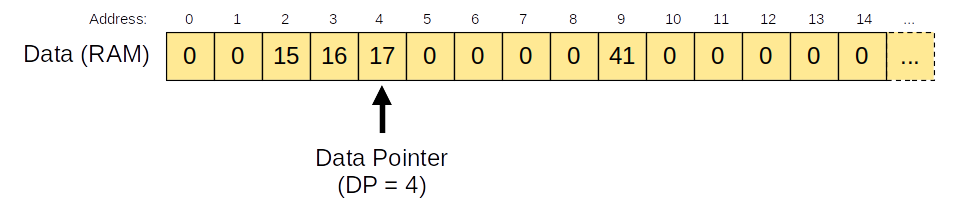
\includegraphics[width=0.9\textwidth]{img/simple_representation}
  \caption{Example state of a BF machine.}
  \label{fig:simplerepresentation}
\end{figure}


The processor consists of three basic building blocks: registers, memory and a control unit. The ALU is missing from this list because the only operations that it needs to perform are addition and subtraction of the value 1, which can be done directly at the register-level when using up/down binary counters like the 74LS193 integrated circuit. The program (a sequence of BF instructions) is stored into Read Only Memory (ROM), whereas the data is stored in Random Access Memory (RAM). Instructions (4-bits) are loaded from ROM into the instruction register (I), together with some flags that encode the state of the machine. Depending on the state and current instruction, the Control Unit sets the appropriate control signals for each of the modules in order for the system to perform the next computation. Figure \ref{fig:architecture} shows how each of the modules is communicating with other modules. In the sections below, each of these connections will be clarified further. The actual implementation on the logic/hardware level is described in section \ref{sec:implementation}.



\begin{figure}[H]
  \centering
  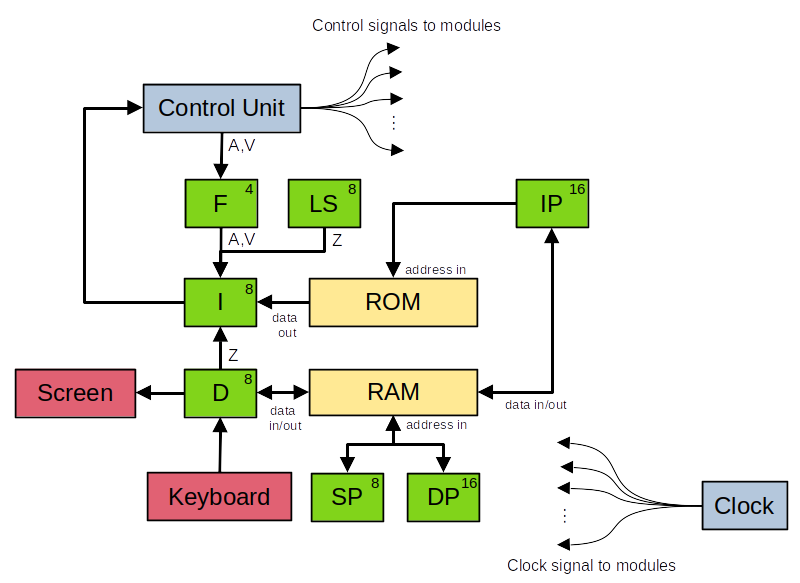
\includegraphics[width=0.9\textwidth]{img/bfcpu_architecture}
  \caption{Connections between modules in the BF processor.}
  \label{fig:architecture}
\end{figure}


\subsection{Data Pointer Register (DP)} \label{sec:architecture:dp}
The data-pointer corresponds to the pointer as specified in the BF-language. It points to some value in memory beyond the stack ($\ge$ 0x0100) and can be either incremented (moved right) or decremented (moved left) using the \texttt{>} and \texttt{<} instructions. Whenever the value pointed to by DP is modified by \texttt{+} or \texttt{-}, it is loaded into the D-register (\ref{sec:architecture:d}), where it can be modified before being stored back into RAM.

\subsubsection*{Inputs}
The DP should be able to increment and decrement (corresponding to the \texttt{<} and \texttt{>} commands), and should be able to be enabled/disabled because of its connection to the address bus of the RAM (the Stack Pointer (SP, see \ref{sec:architecture:sp}, is also connected to this bus). Therefore, the DP has 3 control inputs:
\begin{itemize}
\item EN - Enable - when high, its value is sent to the address bus;
\item INC - Increment - when high, the stored value is incremented on the next clock cycle;
\item DEC - Decrement - when high, the stored value is decremented on the next clock cycle.
\item R - Reset - used to reset only this module to its initial state. This input is only used during initialization, see \ref{seq:sequences:nonbf}
\end{itemize}

\subsubsection*{Outputs}
\begin{itemize}
\item DATA\_OUT - 16 bits, connected to the address bus when enabled (EN high).
\end{itemize}

\subsection{Data Register (D)} \label{sec:architecture:d}
The data register hold a representation of the value currently pointed to by the DP and can be incremented and decremented (corresponding to \texttt{+} and \texttt{-}). The synchronization issue between D and RAM, that results from changing the value in D, is handled by the control unit, as described in section \ref{sec:sequences}.

\subsubsection*{Inputs}
\begin{itemize}
\item DATA\_IN - connected to the data bus;
\item EN - Enable - when high, its value is sent to the data bus;
\item LD - Load - when high, the data on the data bus is loaded into the register on the next clock cycle;
\item INC - Increment - when high, the stored value is incremented on the next clock cycle;
\item DEC - Decrement - when high, the stored value is decremented on the next clock cycle.
\end{itemize}

\subsubsection*{Outputs}
\begin{itemize}
\item DATA\_OUT - 8 bits, connected to the data bus;
\item Z - Zero Flag - high when the register contains all zero's (0x00).
\end{itemize}


\subsection{Instruction Pointer Register (IP)} \label{sec:architecture:ip}
The instruction pointer is a 16-bit value, kept in the IP register, which keeps track of the current instruction that is being executed. It points to a certain address in ROM (which stores the program) and is usually incremented after each instruction has finished executing, in order to move to the next instruction. However, when the processor encounters the \texttt{[}-instruction (and the loop is entered), it needs to store the current value of the IP somewhere in order to be able to jump back to this location. The value is then stored on the stack (the first part of RAM). When the matching \texttt{]}-instruction is encountered, this value is loaded back into the IP instead of simply incrementing the previous value. This has the effect of jumping back in the program, which is how loops are implemented in BF. It is therefore connected to the databus of the RAM in order to be able to store its value on the stack. Because this is not the only register connected to the databus (the other one being the D-register), it needs to be enabled or disabled depending on which of the registers needs access to RAM.

\subsubsection*{Inputs}
\begin{itemize}
\item DATA\_IN - 16 bits - connected to the data bus (for loading a stored address off the stack);
\item EN - Enable - when high, its value is sent to the databus (for storing an address on the stack);
\item LD - Load - when high, the value on the databus is loaded into the register on the next clock cycle;
\item INC - Increment - when high, the stored value is incremented on the next clock cycle.
\end{itemize}

\subsubsection*{Outputs}
\begin{itemize}
\item DATA\_OUT - 16 bits - connected to the databus of RAM and the address inputs of program-ROM;
\end{itemize}


\subsection{Stack Pointer Register (SP)} \label{sec:architecturehitecture:sp}
The stack is the first part of RAM (addresses 0x0000 - 0x00ff) which is reserved to keep track of addresses that might need to be jumped to. The stack-pointer (SP) is incremented whenever a new value is stored on the stack and decremented whenever a value is popped off the stack. In this implementation, the SP is an 8-bit value, which means that at most 256 different values can be stored onto the stack before it the SP overflows (wraps around back to 0) and starts overwriting previous values. This would happen if a BF program was loaded that has more than 256 nested \texttt{[]}-pairs. Although possible, it is very unlikely to happen for the simple programs we intend to run.

\subsubsection*{Inputs}
\begin{itemize}
\item EN - Enable - when high, its value is sent to the address bus;
\item INC - Increment - when high, the stored value is incremented on the next clock cycle;
\item DEC - Decrement - when high, the stored value is decremented on the next clock cycle.
\end{itemize}

\subsubsection*{Outputs}
\begin{itemize}
\item DATA\_OUT - 8 bits - connected to the address bus of RAM.
\end{itemize}

\subsection{Loop Skip Register (LS)} \label{sec:architecture:ls}
The Loop Skip (LS) register is a counter that indicates whether or not we're in the process of skipping a loop. In BF, a loop (\texttt{[}) is only entered when the value currently pointed to is nonzero. In the case that it is zero, execution resumes beyond its matching \texttt{]}. When it is determined (by the Control Unit) that a loop must be skipped (based on the Z-flag of the D-register), the LS register is incremented from 0 to 1. Subsequent instructions are then skipped until either another (nested) loop opening \texttt{[} or a closing \texttt{]} is encountered. On the former, the LS is incremented again while on the latter the LS is decremented. This has the effect that the LS becomes 0 again after the \texttt{]} that matches the original \texttt{[} which led to the skip. Normal execution occurs as soon as LS has become 0 again.

\subsubsection*{Inputs}
\begin{itemize}
\item INC - Increment - when high, the stored value is incremented on the next clock cycle;
\item DEC - Decrement - when high, the stored value is decremented on the next clock cycle.
\end{itemize}

\subsubsection*{Outputs}
\begin{itemize}
\item S - Skip flag - set when the stored data is nonzero. When high, the current instruction should be skipped ($S = \overline{Z}$).
\end{itemize}

\paragraph{Note on preprocessing:} The LS-register is solving a problem that can be avoided by preprocessing the BF code. We could have chosen to somehow include jump-locations in the program and render scanning during runtime (keeping track of the counter to determine when to resume execution) unnecessary. This would however introduce its own set of issues but would also require a fundamental modification to the BF instruction set. We therefore chose not to preprocess the program and require the computer to handle `vanilla' BF.

\subsection{Flag Register (F)} \label{sec:architecture:f}
The sole purpose of the flag register is to buffer the A and V flags, set by the control unit, in case the address or value has changed during the execution of the current instruction. When the next instruction is fetched, these flags are loaded into the instruction register (\ref{sec:architecture:i}). 

\subsubsection*{Inputs}
\begin{itemize}
\item A - Address-change-flag - from CU;
\item V - Value-change-flag - from CU;
\item LD - Load - when high, A and V are latched into the register.
\end{itemize}

\subsubsection*{Outputs}
\begin{itemize}
\item DATA\_OUT - 2 bits - sends the stored A and V flags to the instruction register (\ref{sec:architecture:i}).
\end{itemize}


\subsection{Instruction Register (I)} \label{sec:architecture:i}
The instruction register is an 8-bit register that stores the current instruction, which was loaded from ROM according to the IP value. The BF-instruction itself is only 4 bits wide, which leaves another 4 bits for encoding the state of the machine, using its flags:  A, V, Z and S.

\subsubsection*{Inputs}
\begin{itemize}
\item LD - Load - when high, the current instruction (pointed to by IP) is loaded from program-ROM;
\item Z - Zero-flag - from D;
\item S - Skip-flag - from LS;
\item A - Address-change-flag - from F;
\item V - Value-change-flag - from F.
\end{itemize}

\subsubsection*{Outputs}
\begin{itemize}
\item DATA\_OUT - 8 bits - Sends the current instruction (including flags) to the control unit.
\end{itemize}


\subsection{Memory (RAM)}  \label{sec:architecture:ram}
The RAM stores the data (tape) upon which the BF program is acting (addresses 0x1000 and on). Its second purpose is to provide a stack to store program-addresses on in order to implement conditional loops (0x0000 to 0x00ff). It is connected to both the databus (which in turn connects to D and IP) and to the address-bus (which in turn connects to SP and DP).

\subsubsection*{Inputs}
\begin{itemize}
\item DATA\_IN - 16 bits - connected to the databus (same lines as DATA\_OUT);
\item ADDR\_IN - 16 bits - connected tot the address-bus;
\item OE - Output Enable - the value at the current address is sent to the databus;
\item WE - Write Enable - the value on the databus is loaded into the current address.
\end{itemize}

\subsubsection*{Outputs}
\begin{itemize}
\item DATA\_OUT - 16 bits - connected tot the databus (same lines as DATA\_IN);
\end{itemize}

\subsection{Screen (SCR)}  \label{sec:architecture:scr}
The output module (which is assumed to be a screen) will be attached to the databus and will display whatever is on there when enabled using the Print Enable (PRE) signal.
\subsubsection*{Inputs}
\begin{itemize}
\item EN: Enable Output - Display the contents of D on the next clock pulse.
\end{itemize}

\subsubsection*{Outputs}
None.


\subsection{Keyboard (KB)} \label{sec:architecture:kb}
The input device to the computer is assumed to be a keyboard of some sort, which contains a buffer from which an 8-bit value can be read. Immediately, a design choice has to be made: what happens if the buffer is empty? Either the program continues to run (immediate mode) or the program waits for something to appear in the buffer (buffered mode). The former is convenient for instance when playing games, while the latter is convenient for programs that require user input in order to continue meaningfully. Rather than deciding on either of these modes, we can just implement both. In the microcode table (Table \ref{tab:microcode}, Section \ref{sec:architecture:sequences}) there are two variants of the \texttt{,} command listed (the other one denoted by \texttt{'}), each of which has a different binary representation. When assembling a BF program, we simply pick one or the other and the program should run in the appropriate mode: \texttt{,} for buffered and \texttt{'} for immediate mode.

The buffer of the module should contain all zero's when nothing is present. When running in immediate mode, the programmer should programmatically determine if a value was read and how to act accordingly. In buffered-mode however, after reading from the buffer, the control unit will use the Z-flag to determine whether or not to continue. As long as the value loaded into D is zero, control flow will loop around, trying to get a value from the input buffer. The only control signal going in to the input-module should therefore be the enable-signal, which makes the contents of the buffer available to the databus.

\subsubsection*{Inputs}
\begin{itemize}
\item EN - Enable - sends the contents of the input buffer to the databus.
\end{itemize}

\subsubsection*{Outputs}
\begin{itemize}
\item DATA\_OUT - 8 bits - connected to the databus.
\end{itemize}

\subsection{Control Unit} \label{sec:architecture:cu}
Each of the aforementioned components/modules has one or more control inputs that determine what happens on the next clock cycle. For example, some register-modules can be told to either load a value from their input, increment or decrement the currently stored value, or do nothing at all. It is the Control Unit (CU) that supplies the appropriate control signals to each of the modules before the next clock pulse occurs. The implementation details of how this is done in hardware are discussed in section \ref{sec:implementation}.

Even though the control unit is setting the control signals for all other modules, it has some control signals that it should be able to set for itself. Depending on the instruction that is being executed, it should write values to the flag register. The control signals to indicate that this is being done are called AE and VE respectively. Moreover, its internal instruction counter should be reset in the final cycle of each instruction. This is indicated with the CR (cycle reset) signal.

\subsubsection*{Register Driver} \label{sec:architecture:cu:driver}
Rather that having a seperate signal for each of the INC/DEC-inputs of each register (e.g.~ INC\_D, INC\_LS, etc), a driver module was designed (see \ref{sec:implementation:driver}) to drive the register modules that supports modification of its contents. In addition to a universal INC/DEC signal, three Register Select (RS) bits are used to index the target-register. This approach has two advantages:
\begin{enumerate}
\item It decreases the amount of control signals needed;
\item The logic needed to drive the counting registers (74LS193) only needs to be implemented once.
\end{enumerate}

The driver module accepts 5 control signals: 3 register-select signals (RS0 through RS2), INC and DEC. Using 3 register-select signals, up to 8 ($2^3$) registers can be selected, though only 5 need to be driven by the driver. Table \ref{tab:registers} contains an overview of each of the registers and the control signals they support.

\begin{table}[H]
  \centering
  \begin{tabular}{c|c|c|c|c|c|c}
    Register & \#Bits & EN  & LD  & INC  & DEC & RS \\ \hline 
    D        & 8     & x & x & x & x & 001 \\
    DP       & 16    & x &   & x & x & 010 \\ 
    SP       & 8     & x &   & x & x & 011 \\ 
    IP       & 16    & x & x & x &   & 100 \\ 
    LS       & 8     &   &   & x & x & 101 \\ 
    F        & 4     &   & x &   &   & -   \\ 
    I        & 8     &   & x &   &   & -   \\
  \end{tabular}
  \caption{Control signals available to each of the registers. The F and I register are not connected to the register driver.}
  \label{tab:registers}
\end{table}


\subsubsection*{Inputs}
\begin{itemize}
\item DATA\_IN - 8 bits - current instruction from I;
\item AE - A-flag enable - outputs a high value into the A-bit of the flag register;
\item VE - V-flag enable - outputs a high value into the V-bit of the flag register;
\item CR - Cycle reset - reset the internal cycle counter to 0 to prepare for the next instruction.
\end{itemize}

\subsubsection*{Outputs}
\begin{itemize}
\item RS0 - Register Select, bit 0
\item RS1 - Register Select, bit 1
\item RS2 - Register Select, bit 2
\item INC - Increment selected register
\item DEC - Decrement selected register
\item EN\_D - Enable D
\item EN\_DP - Enable DP
\item EN\_IP - Enable IP
\item EN\_SP - Enable SP
\item OE\_RAM - Output Enable RAM
\item WE\_RAM - Write Enable RAM
\item LD\_D - Load D
\item LD\_IP - Load IP
\item LD\_I - Load I
\item LD\_F - Load F
\item CR - Cycle Reset (CU)
\item VE - V Enable (CU)
\item AE - A Enable (CU)
\item PRE - Print Enable
\item HLT - Halt Clock
\item ERR - Error Signal (CU)
\end{itemize}


